\documentclass[a4paper]{article}

\usepackage[utf8]{inputenc}
\usepackage[spanish,es-tabla]{babel}
\usepackage[T1]{fontenc}
\usepackage{microtype}
\usepackage{newspaper}
\usepackage{multicol}
\usepackage{url}
\usepackage{hyperref}
\usepackage{xcolor}
\hypersetup{
	%% colores de enlaces
	colorlinks,
	linkcolor={red!50!black},
	citecolor={blue!50!black},
	urlcolor={blue!80!black},
	%% metadata del PDF generado
	%% estos metadatos se deben actualizar con cada edición
	pdftitle={Gaceta Galénica - V01E01},
	pdfsubject={Boletín científico del Servicio de Urgencias de la Policlínica Lic. Manuel María Valdés},
	pdfauthor={Moisés Serrano Samudio},
	pdfkeywords={
		Manuel María Valdés,
		fibrilación auricular,
		cardioversión eléctrica,
		cardioversión farmacológica}
}

%% ============================================================================
%% Referencias
%% ============================================================================
\usepackage[
	backend=biber,
	style=nejm,
]{biblatex}

%% Hace que las referencias aparezcan como superíndices
\let\cite=\supercite

%% Añade el documento con referencias bibtex
\addbibresource{referencias.bib}

%% Reduce el tamaño de fuente de las referencias
\renewcommand*{\bibfont}{\scriptsize}

%% ============================================================================
%% Box para viñetas
%% ============================================================================
\usepackage[many]{tcolorbox}
\newtcolorbox{boxClinica}{
	sharpish corners, % better drop shadow
	boxrule = 0pt,
	toprule = 1.5pt, % top rule weight
	enhanced,
	%% {xshift}{yshift}{offset}{step}{options}
	fuzzy shadow = {0pt}{-2pt}{-0.5pt}{0.5pt}{black!35}
}

%% ============================================================================
%% Imágenes
%% ============================================================================
\usepackage{float}
\usepackage{graphicx}
\usepackage{wrapfig}
\usepackage{caption}
\captionsetup[figure]{font=footnotesize}

%% ============================================================================
%% Cabecera
%% ============================================================================
\date{\today}
\currentvolume{1}
\currentissue{1}
\SetPaperName{Gaceta Galénica}
\SetHeaderName{Gaceta Galénica}
\SetPaperLocation{Ciudad de Panamá}
\SetPaperSlogan{''\textit{Ciencia y Verdad}''}
\SetPaperPrice{SU-PMMV}

\newcommand{\NewsAuthor}[1]{%
	\hfill Por \textsc{#1} \vspace{4pt}
	\par \normalfont}

%%
\usepackage{newspaper-mod}
%%
\renewcommand{\headlinestyle}{\itshape\Large\lsstyle}
% \renewcommand{\bylinestyle}{\bfseries\Large\raggedright}
%%

%%%%%%%%%  Front matter   %%%%%%%%%%


\begin{document}

\maketitle

\begin{multicols}{3}


\byline{La Gaceta Galénica}{Moisés Serrano Samudio}

La Gaceta Galénica nace con esta primera edición como una publicación mensual de
la Coordinación de Docencia del Servicio de Urgencias de la Policlínica Lic.
Manuel María Valdés. Es nuestro interés lanzar una edición el primer miércoles
de cada mes con temas cortos dirigidos a mantener actualizados a los colegas
médicos que desempeñan sus labores en los distintos servicios de urgencias
médico-quirúrgicas en instalaciones de primer y segundo nivel de atención en
Panamá.

Se publica como un boletín digital informativo corto, de una a dos páginas de
extensión distribuido por canales digitales. El tema central de la publicación
se presenta acompañado de una viñeta clínica, a partir del cual se discutirán
de manera práctica los aspectos más importantes de la patología abordada con su
respectiva clase y nivel de evidencia.

Planeamos incluir cápsulas históricas sobre la medicina en Panamá y repasar
temas de bioestadística y epidemiología para ofrecer a nuestros lectores
herramientas para refrescar la lectura crítica de la literatura
médico-científica.

Sin más preámbulo, esperamos que disfruten de su lectura tanto como nosotros
disfrutamos preparando el contenido. Feliz lectura.

\closearticle


\headline{¿Quién fue Manuel María Valdés?}

Abogado, economista y periodista. Nace en 1907, proveniente de una familia de
destacados juristas en el ámbito nacional. Nace del matrimonio entre Manuel
María Valdés Arce, quien fue el primer director de los Archivos Nacionales y
hermano de Ramón Maximiliano Valdés Arce, expresidente de la República de
Panamá; y Emma Guardia Vieto que destacaba por un brillante intelecto, hablar
varios idiomas y ser ávida lectora de literatura universal\cite{panamerica10}.

\begin{wrapfigure}{L}{0.18\textwidth}
	\begin{center}
		\vspace{-25pt}
		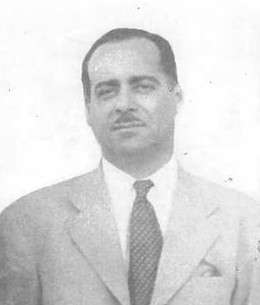
\includegraphics[width=0.17\textwidth]{mmvaldes.jpg}
	\end{center}
	\caption*{Lic. Manuel María Valdés}
\end{wrapfigure}

Al Lcdo. Manuel María Valdés, debemos el honor de la creación de la Caja de
Seguro Social. La gesta que llevo a la fundación de la institución máxima de
la seguridad social en Panamá, tuvo sus albores en 1937 en una reunión en
París entre Arnulfo Arias Madrid y Manuel María Valdés donde intercambiaban
opiniones sobre seguros obligatorios\cite{Pinock95}.

Es la habilidad política y orientación técnica de Don Manuel María Valdés en
conjunto con la tracción del Partido Liberal Unido, que fue fundado por el
expresidente Belisario Porras Barahona, lo que lleva a manos, en aquel entonces,
al Presidente Arnulfo Arias Madrid en 1941 a la firma de la Ley 23 del 21 de
marzo de ese año, publicada en la Gaceta Oficial No. 8481 de marzo de
1941\cite{Pinock95},\cite{gaceta1941}. Nace así la Caja de Seguro Social.

Dedico gran parte de su vida al ejercicio del derecho en los bufetes <<Valdés y
Valdés>>, trabajando junto a su hermano Eduardo Valdés; y <<Valdés, Valdés y
De Castro>>, cuando se asociaron con Woodrow De Castro, otro destacado jurista
panameño.

Fundador de tres diarios: <<El Día>>, <<La Hora>> y <<El Mundo>>. Destacan en
su producción bibliográfica, dos obras: Panamá y su soberanía monetaria (1951),
Intervenciones electorales en Panamá (1932)\cite{Leonard15}.

Fallece en 1968, luego de toda una prolífica carrera. Apodado de cariño Nen,
por sus familiares, amigos, conocidos y sus discípulos del periodismo. Es
despedido en noviembre de ese año\cite{Lot68}.

\closearticle


\headline{Fibrilación atrial: Diagnóstico y manejo}

La fibrilación atrial (FA) es una patología que se ve con regular frecuencia
en los servicios de urgencias. En mayores de 65 años tiene una incidencia
cercana al 10\% y se asocia a una serie de comorbilidades y predispone al
desarrollo de patologías de gran morbimortalidad como el ictus isquémico y el
infarto agudo al miocardio. Se estima una prevalencia para América Latina y El
Caribe en 430 de cada 100000 habitantes\cite{brundel_atrial_2022}.

En Panamá, Pezzullo y colab. estimaron que el 0.9\% de la población adulta
mayor de 20 años es afectada por la FA y que en el año 2015, la FA representó
un costo de 19 millones de Balboas para el sistema de salud
panameño\cite{pezzullo2016}.

\begin{boxClinica}

Paciente masculino de 64 años es traído al servicio de urgencias por personal
de prehospitalaria por síncope con previa historia de palpitaciones, mareos,
debilidad y diaforesis. Sus signos vitales son: PA 160/106 mmHg, FC 141 lpm,
FR 21 cpm, SpO2 92\%, peso 125 kg, estatura 1,65 m. Tiene como antecedentes
importantes tabaquismo y dislipidemia. Se encuentra desorientado y disneico.

\end{boxClinica}

Dentro del abordaje inicial del paciente de la viñeta clínica propuesta, y con
cualquier paciente que se presente con FA a un servicio de urgencias,
el objetivo de tratamiento es lograr la estabilización hemodinámica,
controlar los síntomas y prevenir las complicaciones. Dentro de la
estabilización inicial debemos obtener acceso venoso, O$_{\text{2}}$
suplementario para mantener saturación $\geq$ 92\% y monitorización cardíaca
continua. Hay también que estar preparado para apoyar la ventilación según
sea necesario.

Para establecer el diagnóstico del paciente presentado en la viñeta clínica,
además de la historia clínica y su respectivo examen físico se debe realizar un
electrocardiograma. El ECG tiene una clase y nivel de evidencia IB en FA y es
diagnóstico de FA si un ECG de 12 derivadas o un trazo de 1 derivación
$\geq$ 30 segundos presenta ondas P no discernibles e intervalos RR
irregulares\cite{guiaesc_2021}.

La causa raíz de la FA la encontramos en la electropatología de focos ectópicos
que se ubican el 95\% de las veces en las venas pulmonares. Este sustrato
tisular gatilla la actividad eléctrica en las aurículas de manera irregular
causando la contracción desordenada del tejido muscular en la aurícula. Otros
focos ectópicos encontrados en las venas cavas superior e inferior también
ocasionan un mecanismo eléctrico parecido en las aurículas pero en mucho menor
medida. Las lesiones tisulares subyacentes en las aurículas producto de
isquemia juegan también un papel importante ya que permiten el desarrollo de un
sustrato tisular arritmogénico que lleva también a la despolarización
desordenada de las aurículas. Otro aspecto fisiopatológico destacable son las
alteraciones genéticas que se traducen en mutaciones en canales de sodio,
potasio y calcio que juegan un papel fundamental en la fisiología del ciclo
cardíaco\cite{brundel_atrial_2022}.

Existen una variada clasificación de FA, pero la más aceptada es según
aparición y duración del episodio.

\begin{itemize}
    \item \footnotesize{\textbf{FA diagnosticada por primera vez}: Diagnosticada por primera vez independientemente de duración o gravedad de síntomas.}
    \item \textbf{FA paroxística}: Revierte espontáneamente o con intervención en menos de 7 días.
    \item \textbf{FA persistente}: Con duración mayor a 7 días, aún luego de intervención.
		\item \textbf{FA persistente de larga duración}: Duración mayor a un año, tras adoptar estrategia para control de ritmo cardíaco.
		\item \textbf{FA permanente}: No se adoptan nuevas medidas para control de FA. Representa más una actitud terapéutica del paciente o el médico que atributo fisiopatológico inherente a la FA. Si se realiza una intervención, se reclasifica como FA persistente de larga duración.
\end{itemize}

Los avances en la clasificación, por ejemplo de FA paroxística a FA persistente,
implican un avance en el remodelado estructural auricular o un empeoramiento
de la miocardiopatía auricular.

Se considera al ECG de 12 derivadas como la técnica estándar de diagnóstico en
FA\cite{mairesse2017}. Sin embargo para el cribado un intervención muy
costo-efectiva es la palpación del pulso, esta técnica tiene una sensibilidad
de 87-97\% y especificidad de 70-81\%, esta simple intervención tiene una clase
y nivel de evidencia IB. Es destacable también el uso de monitores de presión
arterial automatizados y el uso de dispositivos \emph{wereables} como relojes
o bandas electrónicas que con sus algoritmos de fotopletismografía ofrecen
también una buena sensibilidad y especificidad, incluso con clase y nivel de
evidencia IB\cite{guiaesc_2021}.

Regresando al paciente de la viñeta clínica, sin antecedentes de FA previa
conocida, habiendo realizado el ECG de 12 derivadas, con toda seguridad nos
encontramos ante un paciente con FA paroxística, pero que está
hemodinámicamente inestable. Es prácticamente mandatorio en este punto,
utilizar el protocolo del ACLS ya que estamos ante un paciente con una
taquicardia inestable, la recomendación aquí según el protocolo ACLS es
cardioversión eléctrica inmediata del paciente, considerando la
sedación previa si fuera necesaria\cite{aha2020}.

% \begin{figure*}[ht]
% 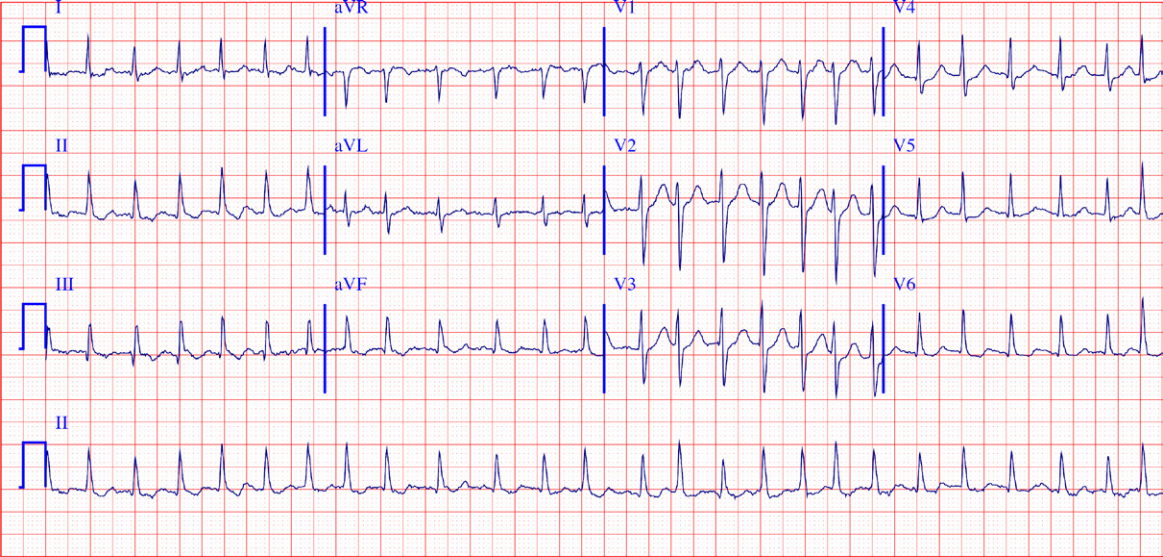
\includegraphics[width=\linewidth]{ecg-fa.png}
% \caption{ECG 12 derivadas. FA de respuesta ventricular rápida}
% \end{figure*}

Según la Guía 2020 de fibrilación auricular de la ESC, la recomendación
con un paciente inestable y con fibrilación atrial es la cardioversión
eléctrica urgente a la máxima dosis permitidida por el
desfibrilador\cite{maxdefib19} e iniciar lo antes posible tratamiento
anticoagulante\cite{guiaesc_2021}, esta recomendación tiene una clase y nivel
de evidencia IB. Luego de la cardioversión eléctrica se puede considerar
la administración de amiodarona para el control inmediato de la frecuencia
cardíaca y esto también puede llevar a una disminución adicional de la
presión arterial\cite{guiaesc_2021}, esta intervención tiene una clase de
recomendación IIb y un nivel de evidencia B, teniendo así evidencia
moderada que la respalde.

Continuando el abordaje de
este paciente, implementamos la estrategia de la vía ABC\cite{lip_abc_2017}.
«A», anticoagulacion / prevención del ictus; «B», buen control de los síntomas;
«C», control de los factores de riesgo cardiovascular y comorbilidades.

Siguiendo la vía ABC, hay que estratificar el riesgo de sufrir un ictus
isquémico o trombótico usando las escales CHA$_{\text{2}}$DS$_{\text{2}}$-VASc
y HAS-BLED respectivamente.

Volviendo a la viñeta clínica, nuestro paciente curso con un episodio de FA
paroxística que fue adecuadamente resuelto.

\closearticle

\printbibliography[heading=none]

\closearticle

\end{multicols}

\end{document}
